% !TEX root = ../main.tex

\section{List of \depms}
\label{app:list}

 %Terminology used includes a central limit order book (CLOB) in which `central' refers to a single orderbook rather than one that is centralized from an operational standpoint. In other words, a decentralized on-chain orderbook can still be called a CLOB. Blockchains are sometimes called layer 1 (L1) chains. An L2 is a faster execution (and generally lower fee) layer that might operate as an optimistic rollup or zk-rollup. An L3... 

\begin{enumerate}

\item \textbf{Bets of Bitcoin} (2011--2014): Centralized event wagering system with BTC as numeraire. Promoted as a prediction market but mechanically it used parimutuel betting. Went offline unannounced with some user funds stuck.

\item \textbf{BitBet} (2012--2020): Centralized event wagering system with BTC as numeraire. Promoted as a prediction market but mechanically it used parimutuel betting. Disruption in 2016 and winddown in 2020. 

\item \textbf{Predictious} (2013--?): Centralized prediction market and CLOB with BTC as numeraire. Promoted as InTrade successor. Appears abandoned in late 2010s.

\item \textbf{Fairlay} (2014--present): Centralized prediction market with BTC as numeraire. Traders were matched on a CLOB (back/lay mechanism). After ownership changes, still operating as Bitcoin Betting. 

\item \textbf{BetMoose} (2014--present) Centralized event wagering system with BTC as numeraire. Promoted as a prediction market but mechanically it used parimutuel betting or back/lay. Still active. 

\item \textbf{Truthcoin / Bitcoin Hivemind} (2014): Decentralized prediction market (\depm) design with follow-up refinements with some code artifacts. Inspired other \depms (particularly around automated book making and token vote market resolution) and sidechain technologies.

\item \textbf{`Princeton' \depm} (2014): Decentralized prediction market (\depm) design as an academic paper only. Inspired other \depms (particularly around share splitting/merging), on-chain CLOBs (frequent batch auctions) and the concept of MEV.  

\item \textbf{Augur} (2015--present): \depm whitepaper design, later deployed on Ethereum (live in 2018) and Polygon (2021). Numeraire is DAI and later USDC. Native token (REP) used in market resolution was one of Ethereum's first ICOs (2015). Still active. Front-ends for Augur include \textbf{Predictions.Global}, \textbf{Veil}, \textbf{Gueser}, and \textbf{Helena Network}.

\item \textbf{BitShares Prediction Markets} (2015--present): \depm functionality was added to the BitShares 2.0 blockchain to support WTA markets and hybrid on/off-chain CLOBs. \depm functionality dormant. BitShares itself is still active but usage has heavily declined.
 
\item \textbf{Gnosis} (2015--present): \depm whitepaper design for Ethereum. Ran closed beta (sight.pm). Pivoted to developing underlying infrastructure for \depms, including the widely used Conditional Tokens Framework (CTF). Co-built Omen based on CTF. Also known for self-custody wallets (Gnosis Safe) and AMM-relevant research (proposing the constant product market maker). Still active. 

\item \textbf{Stox} (2017--2018): Centralized prediction market and CLOB with custom ERC20 token STX as numeraire. Known for celebrity promotions. Abandoned around 2018 after legal issues. 

\item \textbf{Delphy} (2017--?): Prediction aggregator deployed on Ethereum for mobile devices based on points/leaderboard (`play money') rather than money. Appears to have been abandoned within 2-3 years.

\item \textbf{Bodhi} (2017--?): \depm deployed on Qtum blockchain and later Ethereum. Appears to have been abandoned within 2-3 years. 

\item \textbf{BlitzPredict} (2018--2019): Prediction aggregator on Ethereum that appears to have been abandoned before being developed into a full \depm.

\item \textbf{SportX} (2018--): Sports-centric \depm deployed on Ethereum, Polygon, and later its own EVM chain (SX Network). Still active.

\item \textbf{BetProtocol} (2018): Toolkit for \depm infrastructure using custom ERC20 token BEPRO. Bepro Network pivoted in 2021 and no active development on toolkit since.

\item \textbf{Sharpe Capital} (2017--2019): Prediction aggregator on Ethereum that appears to have been abandoned before being developed into a full \depm.

\item \textbf{Amoveo} (\circa 2018--?): \depm functionality into state-channels on a custom PoW L1 chain. Sporadic ongoing development.

\item \textbf{SEER} (2018--?): \depm deployed on custom Graphene-based DPoS L1 chain with custom SEER token as numeraire. Appear abandoned as of 2020.

\item \textbf{Veil} (2019): \depm front-end built on Augur and 0x. Launched and shut down within 2019.

\item \textbf{PredIQt} (2019--?): \depm deployed on EOSIO with IQ/EOS as numeraire. Project pivoted to encyclopedia IQ.wiki and PredIQt appears inactive.

\item \textbf{Catnip.exchange} (2019): \depm front-end for Augur v1 that composed with Balancer AMMs for trading outcome shares. Discontinued after 2020 US presidential election.

\item \textbf{Flux Protocol} (2019--2022): \depm deployed on Ethereum and later NEAR. Appears dormant after 2022. 

\item \textbf{Thales} (2019--2022): Event wagering system deployed on Ethereum and later NEAR. Market resolution with Chainlink. Largely dormant after 2022.

\item \textbf{Omen} (2020--present): \depm built with Gnosis CTF, deployed on Ethereum and later Gnosis Chain (xDai) and Polygon with any ERC20 as numeraire. Market resolution with Reality.eth and Kleros. Still active.

\item \textbf{Polymarket} (2020--present): \depm built with Gnosis CTF, deployed on Polygon with USDC as numeraire. First \depm to receive wide mainstream coverage in the media. Market resolution with UMA. Still active but restricted in some jurisdictions (including the US). 

\item \textbf{PlotX v1} (2020--2022): \depm deployed on Ethereum and later Polygon. Specialized for crypto price predictions. PlotX still active but 2022 pivot left \depm functionality dormant. 

\item \textbf{Reality Cards} (2020--2022): \depm deployed on Ethereum and later Gnosis and Polygon. Outcomes shares are NFTs that can be rented with payouts based on how long a user held the winning NFT (time-weighted to compensate early traders more). Appears abandoned in 2022.

\item \textbf{Prosper} (2021--present): \depm deployed on Avalanche and BSC. Still active.

\item \textbf{Zeitgeist} (2021--present): \depm deployed into the logic of a parachain (custom L1) in the Polkadot/Kusama ecosystem (L0). Still active.

\item \textbf{Polkamarkets} (2021--present): \depm toolkit for EVM chains like Polygon and Moonriver with any ERC-20 as numeraire (and custom ERC20 POLK for governance). Still maintained.

\item \textbf{Hedgehog Markets} (2021--?): Event wagering platform deployed on Solana with USDC as numeraire. Supports both no-loss contests and prediction markets. Appears dormant after 2022.

\item \textbf{Unihedge} (2021): \depm design for EVM with an experimental prototype. Outcomes shares are structured different than a typical prediction market (lots implementing what is known as a Harberger-tax).

\item \textbf{Mojito Markets} (2022--present): \depm designed for Aptos but not yet deployed.

\item \textbf{Insight Prediction} (2024--present): \cepm with blockchain-based payments in various stablecoins, including USDC. Still active.

\item \textbf{Moonopol} (2024--present): \depm deployed on Solana with USDC as numeraire. Still active.

\item \textbf{Miscellaneous}: There are decentralized event wagering systems (or toolkits) that deploy betting structures different from prediction markets. For the earliest systems using such an adjacent approach, we have included them above. However we do not expand on every follow-up project. These include: \textbf{Wagerr}, \textbf{BetDEX}, \textbf{Monaco Protocol}, \textbf{Peerplays}, \textbf{DexWin}, \textbf{DuelDuck}, \textbf{BetterFan}, \textbf{Oriole Insights}, \textbf{BetSwag.gg} and \textbf{Azuro}. We also note here the most prominent \cepms: \textbf{Kalshi}, \textbf{PredictIt}, \textbf{Futuur}, and \textbf{Manifold}. 

\end{enumerate}














\section{Satoshi HBO Market}
\label{app:hbo}

\begin{figure}
  \centering
  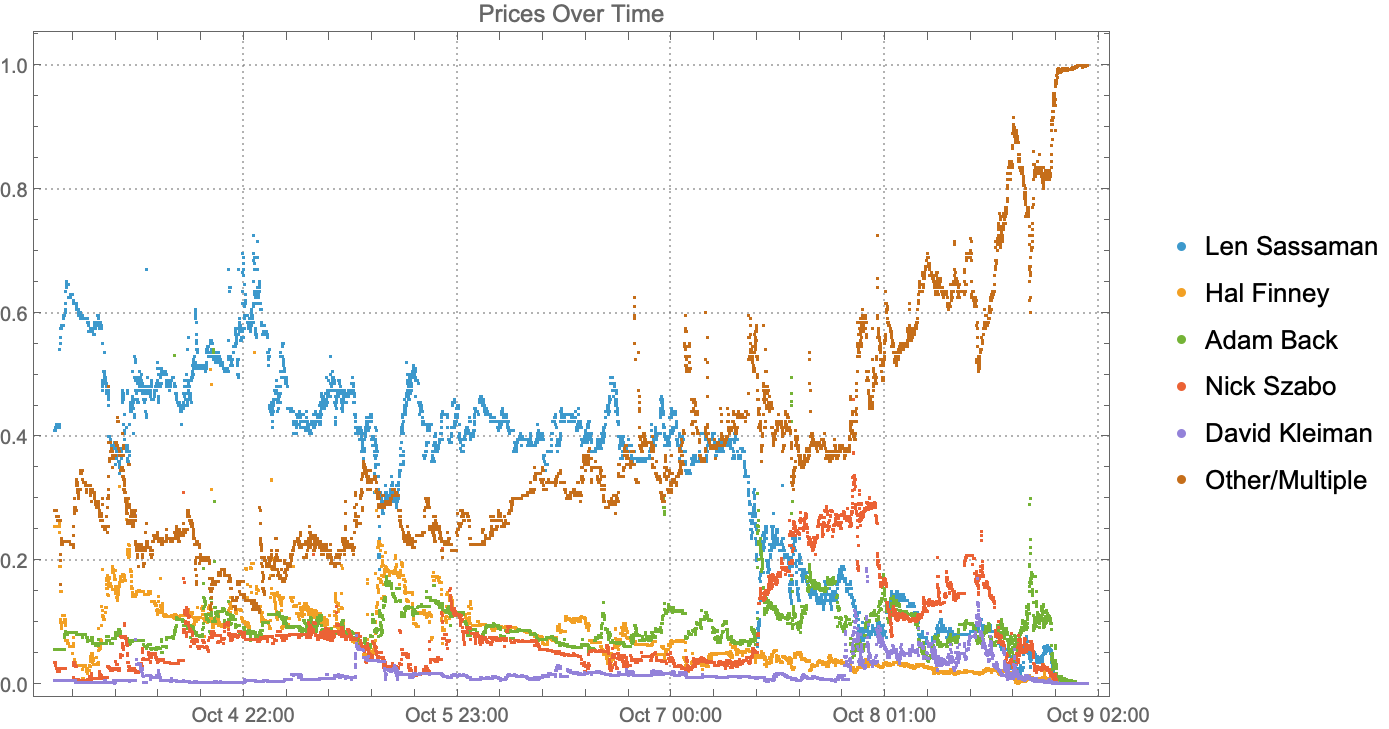
\includegraphics[width=\textwidth]{figures/graph.png}
  \caption{The price movements for 6 leading candidates in the Polymarket market for who would be named as Satoshi Nakamoto in the HBO documentary `Money Electric' which aired the evening of October 8.}
  \label{fig:example}
\end{figure}

\section{Example instantiation of definition}
\label{app:example}

In section~\ref{sec:hbo}, we discussed an example market concerning who the HBO documentary `Money Electric' would name as Satoshi Nakamoto. In this section, we will see how this fits the definitions of a market, prediction market system, and the Arrow--Debreau special case. As discussed in Section~\ref{wf:mech}, Polymarket employs a market mechanism we call a yes/no bundle (YNB), as opposed to winner-take-all (WTA). YNB requires an extra step in the definitions so we will do a first pass with a simplified WTA submarket, and then add the full YNB market.

\subsection{Pass 1: Single WTA Market}

Consider a simplified market that questions whether one specific candidate, \eg Hal Finney, is named as Satoshi: yes or no. If through unforeseen circumstances, who the documentary names is not verifiable by the air date, the market resolves to no.

Recall Definition~\ref{def:market} of a market: 

\begin{definition}[Market]
A (single) market is a tuple $M=(E,\Omega,J,R)$, where $E$ is a well-defined uncertain event, $\Omega$ is a nonempty outcome space for $E$, $J$ is a finite index set of contract labels (“shares”), and $R=(R_j)_{j\in J}$ are nonnegative payoff functions with $R_j:\Omega\to\mathbb{R}_{\ge 0}$. 
We assume $|J|\ge|\Omega|$ and we require \emph{outcome distinguishability} on $\Omega$:
\[
\forall\,\omega\neq\omega'\in\Omega\ \ \exists\,j\in J:\ R_j(\omega)\neq R_j(\omega').
\]
When $M$ resolves to $\omega_M\in\Omega$, one unit of share $j\in J$ pays $R_j(\omega_M)$ (in units of $\mathcal{N}$ defined below).
\end{definition}

Event $E$ is whether or not Hal Finney is named as Satoshi in the documentary.

$\Omega$ is the set of resolution outcomes the market recognizes for $E$—the labels the system can publish at settlement. For this Hal-only binary market the outcome space is $\Omega=\{\mathsf{True},\mathsf{False}\}$. Here $\mathsf{True}$ means the documentary (per the market’s stated criteria) identifies Hal Finney as Satoshi; $\mathsf{False}$ aggregates all other possibilities (Hal not named, someone else named, no one named, the film does not air, or the identification is not verifiable by the resolution deadline).

%Once some $\omega\in\Omega$ is published, all payoffs $R_j(\omega)$ are determined.

We require that $\Omega$ contain no redundant labels. A label is redundant if it does not change at least one contract’s payoff: $\omega\sim\omega' \iff \forall j\in J,\ R_j(\omega)=R_j(\omega')$. For example, “Hal is named and it is raining’’ and “Hal is named and it is not raining’’ are distinct real-world states, but they cannot both appear in $\Omega$ since they both map to $\mathsf{True}$. The restriction can be written as:
\[
\forall\,\omega\neq\omega'\in\Omega\ \ \exists\,j\in J:\ R_j(\omega)\neq R_j(\omega').
\]

In a prediction market, there are a set of shares. If we label them and add them all to an index set, that set is $J$. For this example, $J=\{\textsf{YES},\textsf{NO}\}$: Hal Finney is named (yes) and else (no). This is a normal case where each share in $J$ corresponds to an outcome in $\Omega$ but it is possible that the number of shares could exceed the number of outcomes.\footnote{For example, consider a market of where Newcastle United (NUFC) finishes in the 2024-35 English Premier League season. Since there are 20 teams, the outcome has 20 possible labels: positions 1 to 20. Shares could exist for each of the 20 positions. But the outcome could also settle shares for whether NUFC finishes in the top 5 (which is relevant to champions league admittance), or shares on finishing in the bottom 3 (which is relevant to relegation).}

$J$ is the index set of contract labels—the names of the tradeable shares. In this binary market we take $J=\{\textsf{YES},\textsf{NO}\}$. 

The labels get their meaning from the component payoff functions $R_j:\Omega\to\mathbb{R}_{\ge 0}$. In this example, a payoff of 1 is given for shares that correctly predict the outcome and 0 otherwise. This means $R_{\textsf{YES}}(\mathsf{True})=1$, $R_{\textsf{YES}}(\mathsf{False})=0$, $R_{\textsf{NO}}(\mathsf{True})=0$, $R_{\textsf{NO}}(\mathsf{False})=1$.

Recall Definition~\ref{def:market} of a prediction--market system $\mathcal{S}=(\mathcal{M},\mathcal{N},\mathsf{Res})$:
$\mathcal{M}$ is the (countable) catalog of markets; $\mathcal{N}$ is the numeraire (unit of account used to price and settle claims);
and $\mathsf{Res}=\{\mathrm{res}_M\}_{M\in\mathcal{M}}$ assigns to each market $M$ a resolution register that is initially
$\bot$ and flips exactly once to some $\omega_M\in\Omega_M$.
When $\mathrm{res}_M\neq\bot$, we set $\omega_M:=\mathrm{res}_M$ and each unit of label $j\in J$ settles for $R_j(\omega_M)$ units of $\mathcal{N}$.

This market is a winner--take--all (Arrow--Debreu) special case: there is a bijection $\iota:J\to\Omega$ as follows: $\textsf{YES}\rightarrow\mathsf{True}$ and $\textsf{NO}\rightarrow\mathsf{False}$. Payoffs are $R_j(\omega)=\mathbf{1}\{\omega=\iota(j)\}$. Hence, for each $\omega\in\Omega$, exactly one label pays $1$ and all others pay $0$. 

The market tuple $M=(E,\Omega,J,R)$ specifies \emph{what} to pay \emph{given} an outcome (via $R$).
The register $\mathrm{res}_M$ is the system’s single source of truth for \emph{which} outcome actually occurred:
before resolution $\mathrm{res}_M=\bot$ (no settlement), after resolution $\mathrm{res}_M=\omega_M\in\Omega_M$ (settlement applies).

Polymarket instantiates $\mathcal{S}$ with $\mathcal{M}$ equal to its live and historical markets, $\mathcal{N}$ the USD–denominated stablecoin USDC, and $\mathsf{Res}$ implemented by its on–chain resolution process (e.g., UMA’s optimistic oracle) that writes a single outcome to each $\mathrm{res}_M$.

For the Hal–only binary market, the system maintains a resolution register
$\mathrm{res}_{M_{\mathrm{Hal}}}\in\{\bot\}\cup\Omega$ with
$\Omega=\{\mathsf{True},\mathsf{False}\}$ (i.e., “yes/no” to the proposition).
The register is initially $\bot$ and, after the platform’s resolution process completes, the oracle writes a single value
$\omega_{M_{\mathrm{Hal}}}\in\Omega$ to the register.

Set $\omega_{M_{\mathrm{Hal}}}=\mathsf{True}$ iff the documentary (per stated criteria) identifies \emph{Hal Finney} as Satoshi; otherwise set $\omega_{M_{\mathrm{Hal}}}=\mathsf{False}$.

Shares are fully collateralized to \$1 in the numeraire $\mathcal{N}$ (USDC): a unit of \textsf{YES} pays $1$\,USDC at $\mathsf{True}$ and $0$\,USDC at $\mathsf{False}$; a unit of \textsf{NO} pays $1$\,USDC at $\mathsf{False}$ and $0$\,USDC at $\mathsf{True}$. Formally,
\[
R_{\textsf{YES}}(\mathsf{True})=1,\ \ R_{\textsf{YES}}(\mathsf{False})=0,\qquad
R_{\textsf{NO}}(\mathsf{True})=0,\ \ R_{\textsf{NO}}(\mathsf{False})=1.
\]

In the aired documentary, \emph{Peter Todd} was named; therefore
\[
\mathrm{res}_{M_{\mathrm{Hal}}}=\omega_{M_{\mathrm{Hal}}}=\mathsf{False},
\]
and each unit settles as
\[
\textsf{YES}\ \to\ 0\ \text{USDC},\qquad
\textsf{NO}\ \to\ 1\ \text{USDC}.
\]

% = = = 

\subsection{Pass 2: YNB Market}

We define a \textit{family} of markets $\{M_c\}_{c\in C}$ where each $c\in C$ names one market in the family. For the HBO film, $C$ is the set of candidates including $\mathsf{Finney}$, $\mathsf{Szabo}$,  $\mathsf{Sassaman}$,  $\mathsf{Back}$, and $\mathsf{Other/Multiple}$. The event $E_c$ for a particular $\{M_c\}$ is: the documentary identifies $c$ as Satoshi. For each candidate's market, the relevant market outcomes are $\Omega_c=\tuple{\mathsf{True},\mathsf{False}}$. As a YNB market, Polymarket creates a yes share and a no share for each candidate $J_c=\tuple{\textsf{YES},\textsf{NO}}$ called a yes/no bundle (YNB). The payoffs are as follows: $R^{(c)}_{\textsf{YES}}(\mathsf{True})=1$, $R^{(c)}_{\textsf{YES}}(\mathsf{False})=0$, $R^{(c)}_{\textsf{NO}}(\mathsf{True})=0$, and $R^{(c)}_{\textsf{NO}}(\mathsf{False})=1$. Each $\{M_c\}$ has its own volume of outstanding shares, its own pricing, and its own orderbook or AMM. 

For settling, $\mathsf{Res}=\{\mathrm{res}_{M}\}_{M\in\mathcal{M}}$ gives each $M_c$ a register $\mathrm{res}_{M_c}\in\{\bot\}\cup\Omega_c$, initially $\bot$, that flips exactly once to $\omega_{M_c}\in\Omega_c$. The documentary named Peter Todd, who was not one of the named candidates and thus fell under \textsf{Other/Multiple}: $\omega_{M_{\textsf{Other/Multiple}}}=\mathsf{True}$ while $\omega_{M_c}=\mathsf{False}$ for all other $c\neq\textsf{Other/Multiple}$. 

The $R^{(c)}_j(\omega_{M_c})$ for \textsf{Other/Multiple: YES} was $1$ USDC, \textsf{Other/Multiple: NO} was $0$ USDC, every other named candidate’s \textsf{NO} paid $1$ USDC and their corresponding \textsf{YES} paid $0$ USDC. 

% = = = 

\subsection{Axioms}

Polymarket works through \textit{splitting} (see \S\ref{wf:trade}) as follows. Any trader can receive 1 yes share and 1 no share for a specified candidate's market $\{M_c\}$  by depositing 1 USDC into the treasury for the market. When the market resolves, one share will resolve for 1 USDC and one will resolve for 0 USDC. Thus in both cases, Polymarket has exactly the correct amount in the treasury to complete its payout and is solvent. Every split increases the number of shares (yes and no) by 1 share and increase the treasury by 1 USDC. After the market resolves, the winning shares can be redeemed for 1 USDC which decreases the outstanding winning shares by 1 and reduces the treasury by 1 USDC. Shares are fungible as the payout for each share of the same type is identical. Polymarket allows shares to withdrawn as ERC20 tokens and traded using any compatible marketplace. It also provides a CLOB and an AMM for each share.

The HBO documentary market is a special case, called negative risk (NR), in which each candidate's yes/no bundle is a complete set of outcomes (either the candidate is named or the candidate is not named) and additionally the set of yes shares for each candidate is complete (one and only one of the candidates will be declared the winner). Thus it is WTA across each yes/no bundle and it is also WTA across all yes shares.

